%! Tex program = xelatex
\documentclass{article}

%\usepackage[UTF8]{ctex}
\usepackage{amsmath,amssymb}
\usepackage{ntheorem}
\usepackage[letterpaper,top=2cm,bottom=2cm,left=3cm,right=3cm,marginparwidth=1.75cm]{geometry}%table package
%Table
\usepackage{multirow,booktabs}
\usepackage{makecell}
%字体颜色
\usepackage{color}
\usepackage[dvipsnames]{xcolor}  % 更全的色系
%代码
\usepackage[OT1]{fontenc}
\usepackage[framed,numbered,autolinebreaks,useliterate]{/Users/anye_zhenhaoyu/Desktop/Latex/mcode}
\usepackage{listings}
\usepackage{algorithm}
\usepackage{algorithmic}
%插图
\usepackage{graphicx}
%改变item格式
\usepackage{enumerate}
%物理
\usepackage{physics}
%extra arrows
\usepackage{extarrows}
% caption
\usepackage[justification=centering]{caption}
% htpb
\usepackage{stfloats}

\def\RR{\mathbb{R}}
\def\ZZ{\mathbb{Z}}
\def\EE{\mathbb{E}}

\def\Trsp#1{#1^{\mathcal{T}}}

\def\bw{\boldsymbol{\omega}}
\def\ba{\boldsymbol{a}}
\def\bb{\boldsymbol{b}}
\def\bc{\boldsymbol{c}}
\def\bd{\boldsymbol{d}}
\def\bt{\boldsymbol{t}}
\def\bx{\boldsymbol{x}}
\def\by{\boldsymbol{y}}
\def\bz{\boldsymbol{z}}

\def\bA{\boldsymbol{A}}
\def\bB{\boldsymbol{B}}
\def\bC{\boldsymbol{C}}
\def\bE{\boldsymbol{E}}
\def\bO{\boldsymbol{O}}
\def\bX{\boldsymbol{X}}
\def\bY{\boldsymbol{Y}}

\def\Esolve{\textcolor{blue}{Solve: }}
\def\Eproof{\textcolor{blue}{Proof: }}

\def\suminf#1{\sum_{#1=-\infty}^{+\infty}}

\newtheorem{lemma}{Lemma}
\newtheorem{proof}{Proof}
\newtheorem*{theorem}{Theorem}

\graphicspath{{hw6/figures/}}

\begin{document}
\title{Homework 6}
\author{Zhen}
\maketitle


\section*{Problem 1}
\begin{enumerate}[(a).]

	\item Considering that $\nabla^2f=Q$, the eigenvalues of $\nabla^2f$ is $\gamma$ and $1$.

		So we have $\max\qty{\gamma,1}\le \abs{L}$. Then the smallest $L$ such that $f$ is $L$-smooth is $\max\qty{\gamma,1}$.

	\item 
		$f(\bx)-\dfrac{m}{2}\norm{\bx}^2=
		\dfrac{\gamma-m}{2}x_1^2+
		\dfrac{1-m}{2}x_2^2$ is convex.
		Thus $diag(\dfrac{\gamma-m}{2},\dfrac{1-m}{2})\succeq \bO$.

		Finally we have $m\le \min(\gamma,1)$.
	\item
		When the step size is 1, 0.1 and 0.01, $\bx_0$ converges. While for the size 2.2, it does not converge.
		\begin{table}[h]
			\centering
			\begin{tabular}{c|c|c|c}
				step sizes & Num of Iter & step sizes & Num of Iter \\
				2.2 & NaN & 1 & 88 \\
				0.1 & 917 & 0.01 & 9206 \\
			\end{tabular}
			\caption{Number of Iteration}
		\end{table}

		\begin{figure}[h]
		\centering
		\begin{minipage}[b]{0.23\linewidth}
			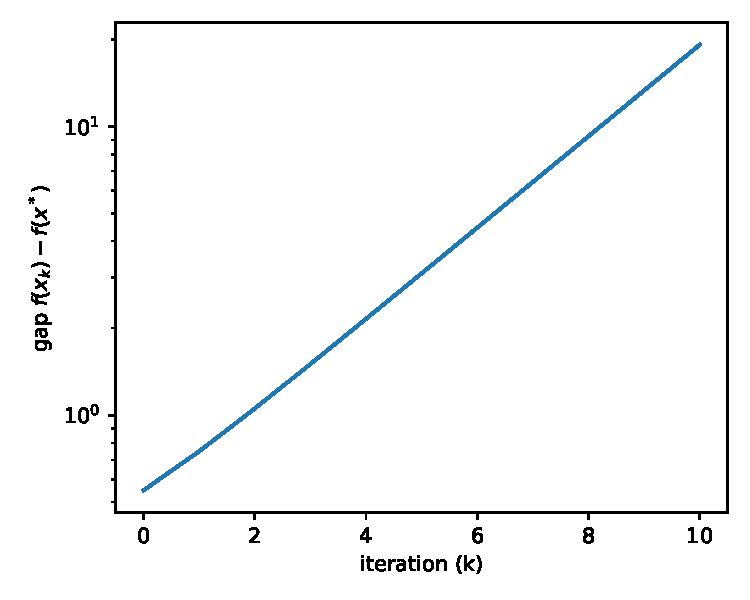
\includegraphics[width=1\linewidth]{gd_f_gamma0.1_ss2.2.pdf}\vspace{4pt}
			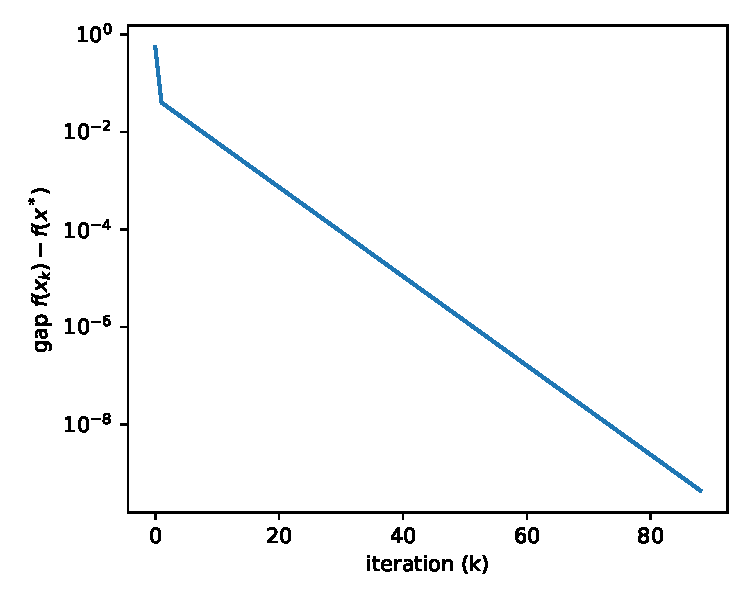
\includegraphics[width=1\linewidth]{gd_f_gamma0.1_ss1.pdf}
		\end{minipage}
		\begin{minipage}[b]{0.23\linewidth}
			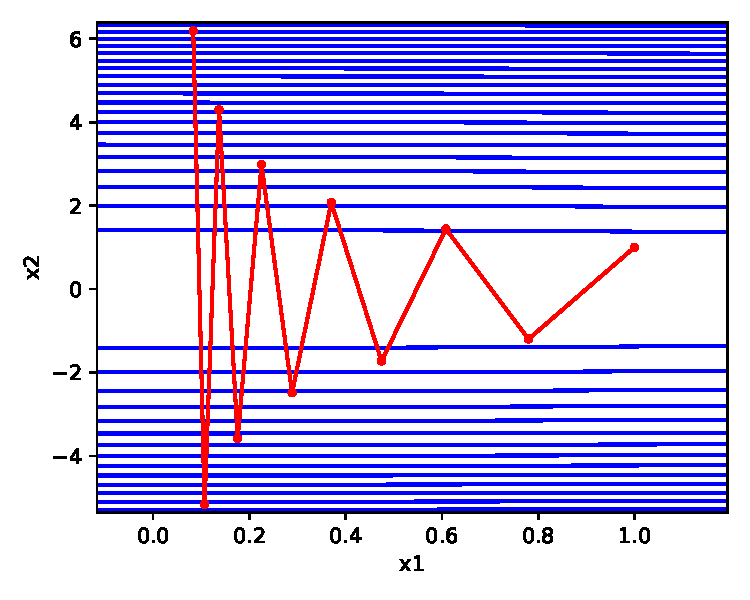
\includegraphics[width=1\linewidth]{gd_traces_gamma0.1_ss2.2.pdf}\vspace{4pt}
		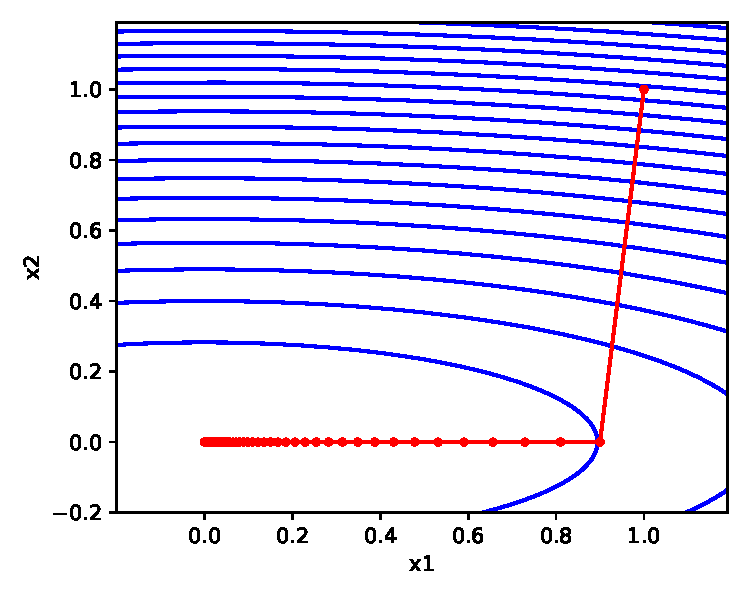
\includegraphics[width=1\linewidth]{gd_traces_gamma0.1_ss1.pdf}
		\end{minipage}
		\begin{minipage}[b]{0.23\linewidth}
			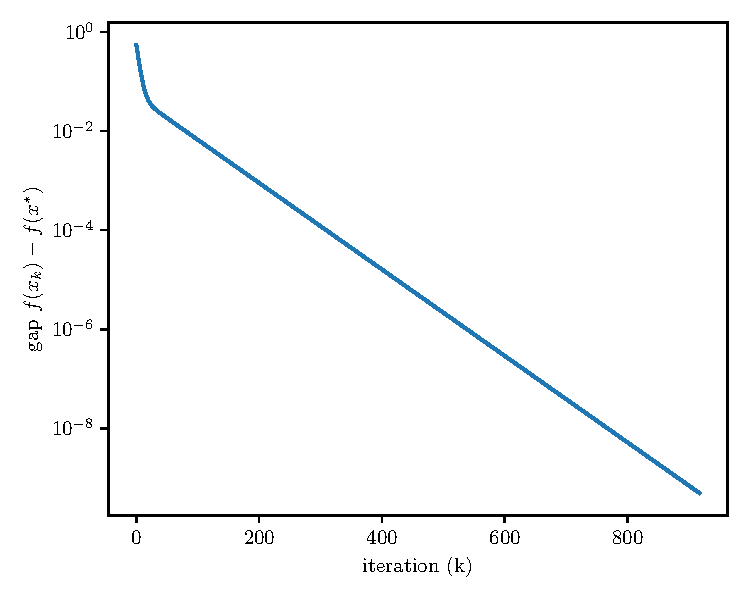
\includegraphics[width=1\linewidth]{gd_f_gamma0.1_ss0.1.pdf}\vspace{4pt}
		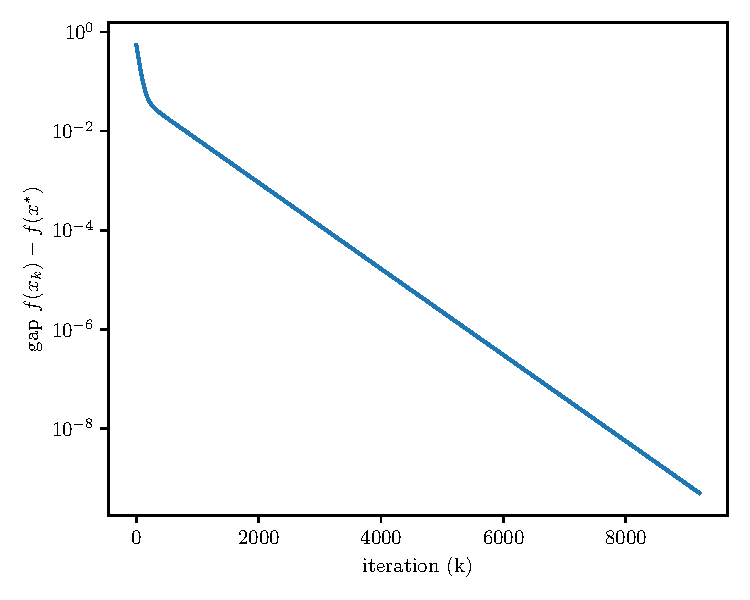
\includegraphics[width=1\linewidth]{gd_f_gamma0.1_ss0.01.pdf}
		\end{minipage}
		\begin{minipage}[b]{0.23\linewidth}
			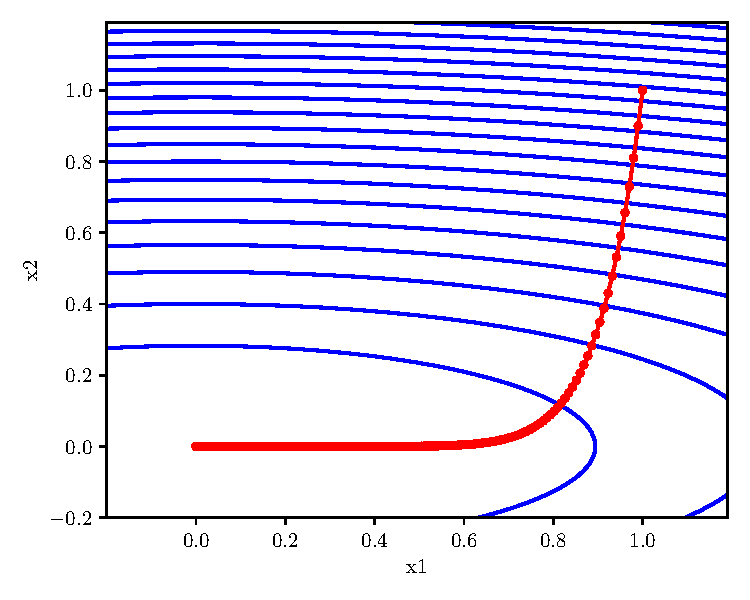
\includegraphics[width=1\linewidth]{gd_traces_gamma0.1_ss0.1.pdf}\vspace{4pt}
			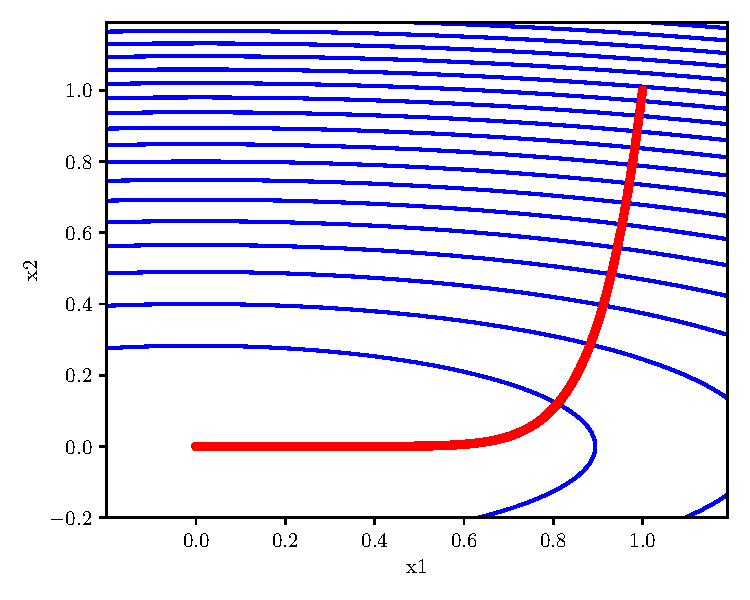
\includegraphics[width=1\linewidth]{gd_traces_gamma0.1_ss0.01.pdf}
		\end{minipage}
		\caption{The step size of each case are:\\
		upper left: 2.2, upper right 0.1, bottom left: 1.0, bottom right: 0.01}
		\end{figure}

		The output is:
		\begin{figure}[h]
			\centering
			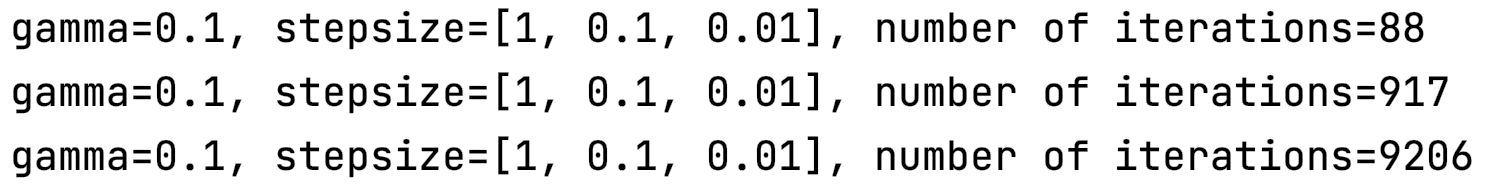
\includegraphics[width=0.7\linewidth]{p1c.png}
			\caption{The Output of P1(c)}
		\end{figure}

		\newpage
	\item
		The output of each case is as follows.
		\begin{figure}[h]
			\centering
			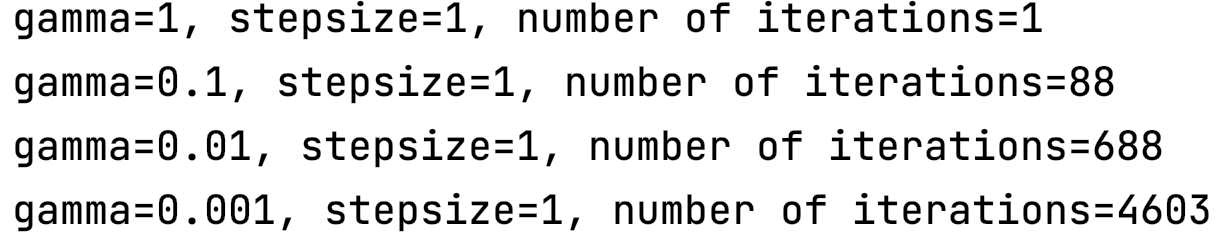
\includegraphics[width=0.7\linewidth]{p1d.png}
		\end{figure}

		By the figure we have: when $\gamma\downarrow$, iterations $\uparrow$.
\end{enumerate}


\section*{Problem 2}

Let the stepsize be $0.2$ and finally we get:
\begin{figure}[h]
	\centering
	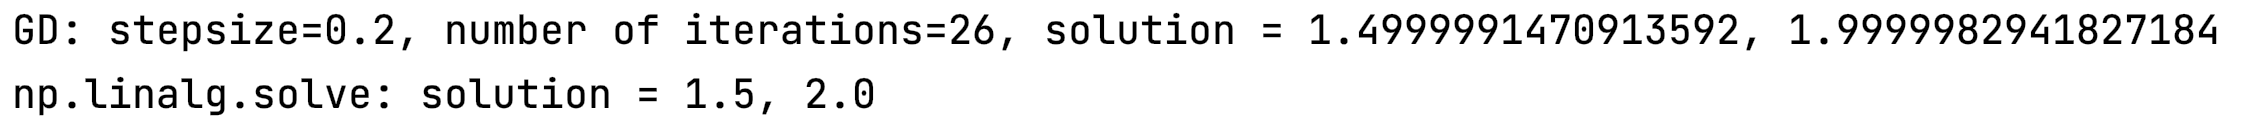
\includegraphics[width=0.9\linewidth]{p2.png}
	\caption{The Output of P2}
\end{figure}
\\
\textcolor{blue}{Answer:} $\bw=(1.5000,2.0000)^{\mathcal{T}}$.

Apparently they agree with each other.

\section*{Problem 3}

The output is:
\begin{figure}[h]
	\centering
	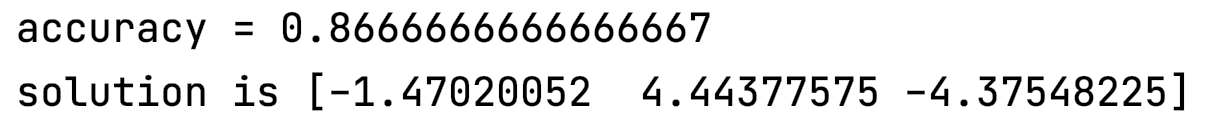
\includegraphics[width=0.5\linewidth]{p3.png}
\end{figure}
\\
Then we could get the visualization

\begin{figure}[H]
	\centering
	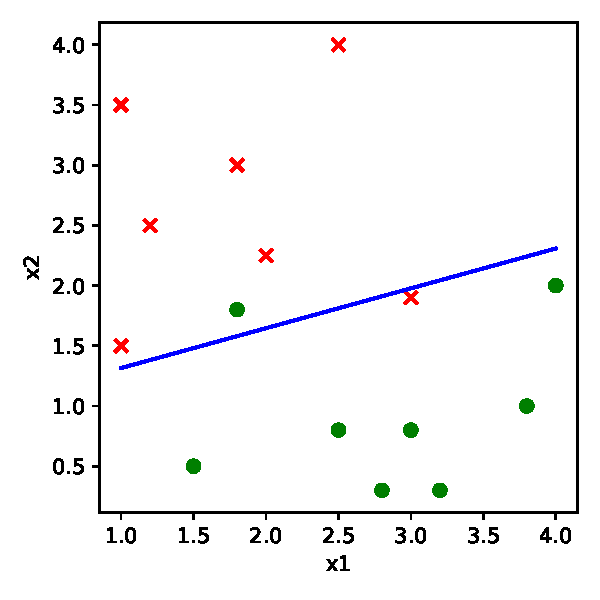
\includegraphics[width=0.5\linewidth]{p3.pdf}
\end{figure}
\\
\textcolor{blue}{Answer:} $\bw = (-1.470,4.444,-4.375)^{\mathcal{T}}$, $Acc = 0.8667$
\newpage
\section*{Problem 4}
Suppose $f(\bx)$ is differentiable and $\alpha$-strongly convex, and $g(\bx)$ is $\beta$-smooth. Show that the function $h(\bx) = f(\bx)-g(\bx)$ is convex if $\alpha \ge \beta$.
\\

\Eproof
\\
By the premise we have:
\\
\\
$f(\bx)-\dfrac{\alpha}{2}\norm{\bx}^2$ is convex which means that 
$$f(\bx)-\dfrac{\alpha}{2}\norm{\bx}^2 \ge f(\by)-\dfrac{\alpha}{2}\norm{\by}^2 + \Trsp{(\nabla f(\by)-\alpha\by)}(\bx-\by)$$
\\
Also, because $h$ is $\beta$-smooth,
$$
h(\bx)\le h(\by)+\nabla h(\by)^{\mathcal{T}}(\bx-\by)+\dfrac{\beta}{2}\norm{\bx-\by}^2
$$

Rearrange 2 above equations:

\begin{equation}
	\nabla f(\by)^{\mathcal{T}}(\bx-\by)
	\le
	f(\bx)-f(\by)-\frac{\alpha}{2}\norm{\bx-\by}^2
\end{equation}
and
\begin{equation}
-\nabla h(\by)^{\mathcal{T}}(\bx-\by)
\le
-h(\bx)+h(\by)+\dfrac{\beta}{2}\norm{\bx-\by}^2
\end{equation}

Plugging Eq(1) and Eq(2):

$$
\begin{aligned}
	\qty(\nabla f(\by)-\nabla g(\by))^{\mathcal{T}}(\bx-\by)
	&\le
	f(\bx)-g(\bx)-f(\by)+g(\by)+\dfrac{\beta-\alpha}{2}\norm{\bx-\by}^2
	\\
	&\le
	f(\bx)-g(\bx)-f(\by)+g(\by)
\end{aligned}
$$

Rearrange the above Eq.:
$$
\begin{aligned}
	&
	f(\bx)-g(\bx)\ge f(\by)-g(\by)+\qty(\nabla f(\by)-\nabla g(\by))^{\mathcal{T}}(\bx-\by)
	\\
	\iff
	&
	h(\bx)\ge h(\by)+\nabla h(\by)^{\mathcal{T}}(\bx-\by)
	\\
	\iff
	&
	h(\bx) \mbox{ is convex.}
\end{aligned}
$$

\end{document}

